\subsection{Previous work}

\subsubsection{Mixed-Initiative Co-Creativity}
Similar to user or player modeling, designer modeling for content creation tools (CAD and MI-CC tools) was suggested by Liapis et al~\citepfifth{p5Liapis2013-designerModel}, where it is proposed the use of designers models that capture their styles, preferences, goals, intentions, and interaction processes. In their work, they suggest methods, indications, and advice on how each part can be model to be integrated into a holistic designer model, and how each game facet can use and benefit from designer modeling. Moreover, in \citepfifth{p5Liapis2014-designerModelImpl} the same authors discuss their implementation of designer modeling and the challenges of integrating all together in their MI-CC tool, Sentient Sketchbook, which had a positive outcome on the adaptation of the tool towards individual “artificial” users.

Furthermore, Lehman et al \citepfifth{p5lehman2016creative} presented Innovation Engines that combine the capabilities and advantages of machine learning and evolutionary algorithms to produce novel 3D graphics with the use of Compositional Pattern-Producing Networks (CPPN) evolved with MAP-Elites, and evaluated by the confidence a deep neural network had on the models belonging to a specific object category.

\subsubsection{Procedural Content Generation via Machine Learning}
Summerville et al. \citepfifth{p5summerville2018procedural} define Procedural Content Generation via Machine Learning (PCGML) as the generation of game content by models that have been trained on existing game content. The main approaches to PCGML are: autonomous content generation, content repair, content critique, data compression, and mixed-initiative design.

\begin{figure}
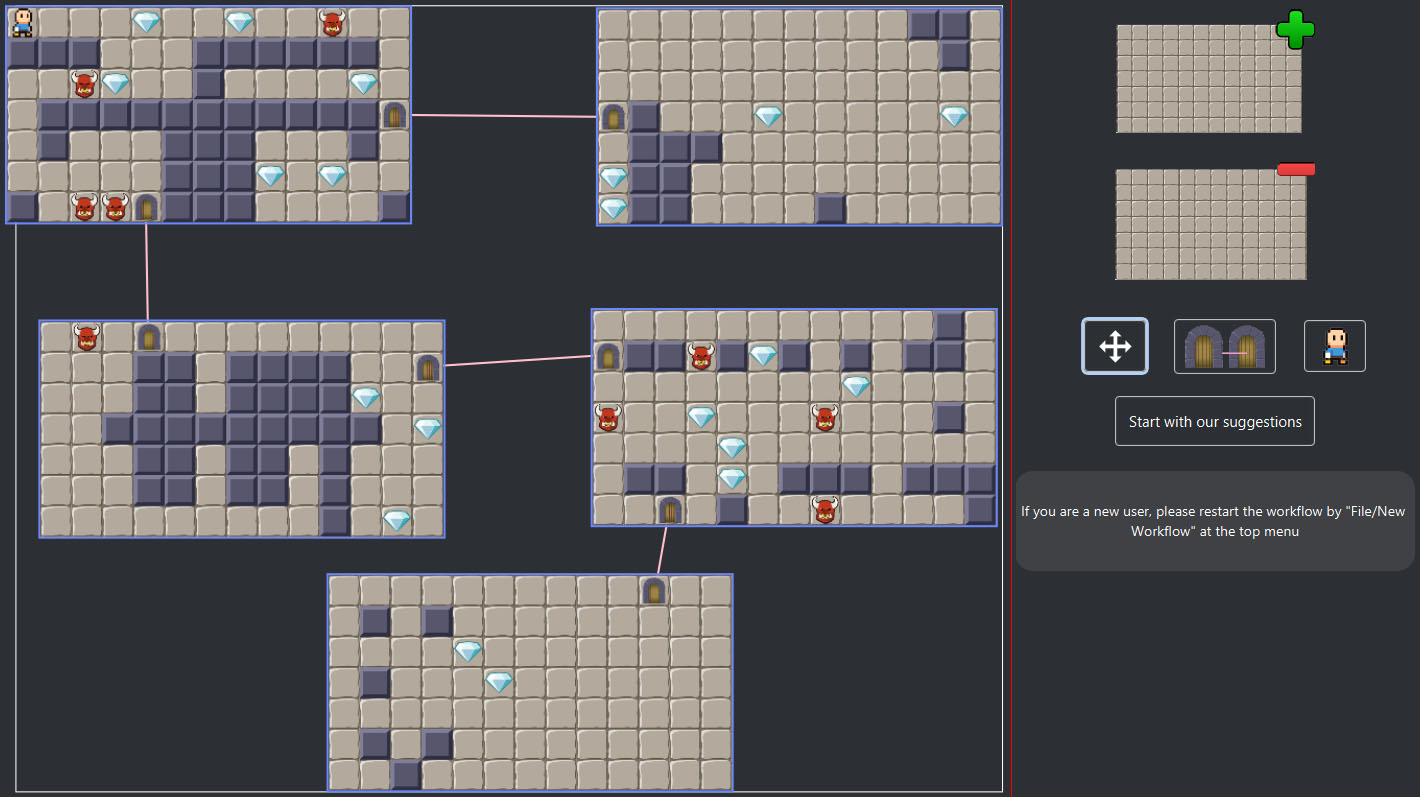
\includegraphics[width=\textwidth]{fig1.jpg}
\caption{Screenshot of the dungeon editor screen in EDD, displaying a sample dungeon composed by five rooms.} \label{p5fig1}
\end{figure}

In the latter case and, as appointed by Treanor et al. \citepfifth{p5treanor2015ai}, AI may engage with a human user participating in the creation of content, so that new gameplay emerges from this shared construction. This emerging relationship between the user and the AI system, when implemented through a trained machine learning algorithm, has the potential to reduce user frustration, error, and training time. This is due to the capacity of a machine learning solution to adapt to the design preferences of the user that interacts with the MI-CC tool by learning from the user-generated dataset of previous choices.

\subsubsection{The Evolutionary Dungeon Designer}

The Evolutionary Dungeon Designer (EDD) is an MI-CC tool for designers to build 2D dungeons. EDD allows designers to manually edit the overall dungeon and its composing rooms (see Figure \ref{p5fig1}), as well as to use procedurally generated suggestions either as inspiration to work on or as a finished design (see Figure \ref{p5fig2}). Both options fluently alternate during the creation process by means of a workflow of mutual inspiration, through which all manual editions performed by the user are fed into the underlying continuous Evolutionary Algorithm, accommodating them into the procedural suggestions. A detailed description of EDD and its features can be found in~\citepfifth{p5Alvarez2018a,p5Alvarez2018,p5Baldwin2017a,p5Baldwin2017}.

Subsequent user studies \citepfifth{p5Alvarez2018,p5Baldwin2017} carried out with game designers on EDD raised the following areas of improvement: (1) the designers struggled with EDD’s capability of understanding the designer’s intentions and preserving custom designs; (2) the tool was unable to generate aesthetically pleasing suggestions since the fitness function only accounted for functionality, but not aesthetics, of design patterns; (3) the designers wanted to keep certain manual editions from being altered by the procedural suggestions.  

With the aims of addressing these limitations as well as fostering the user's creativity with quality-diverse proposals, EDD was improved with the Interactive Constrained MAP-Elites (IC MAP-Elites) \citepfifth{p5alvarez2019empowering}, an implementation of MAP-Elites into the continuous evolutionary process in EDD. With this addition, the user drives the generation of procedural suggestions by modifying at any moment the areas of the search space where the evolution should put the focus on. This is done by selecting among the available dimensions: symmetry, similarity, design patterns, linearity, and leniency. Additionally, the designers have now the chance to limit the search space by locking map areas and thus preserving manually edited content.

This paper contributes by building on top of EDD's IC MAP-Elites, adding a data-driven Designer Preference Model that adapts and personalizes the design experience, as well as balances the expressivity of the tool and the controllability of the designer over the tool. Other researchers have pursued a similar goal by biasing the search space through having the user perform a manual selection after every given number of generations~\citepfifth{p5Picbreeder-Secretan2008,p5Liapis2012-adaptiveVisual,p5Novelty-Lehman2011}. Nevertheless, this approach leads to an increase in user fatigue by repeatedly asking for user input and thus, stalling the evolutionary process until such input is received. Moreover, this staged process seems incompatible with the dynamic reciprocal workflow of MI-CC tools, where the focus is on the designer proactively creating content rather than passively browsing a set of suggestions.

\begin{figure}[t]
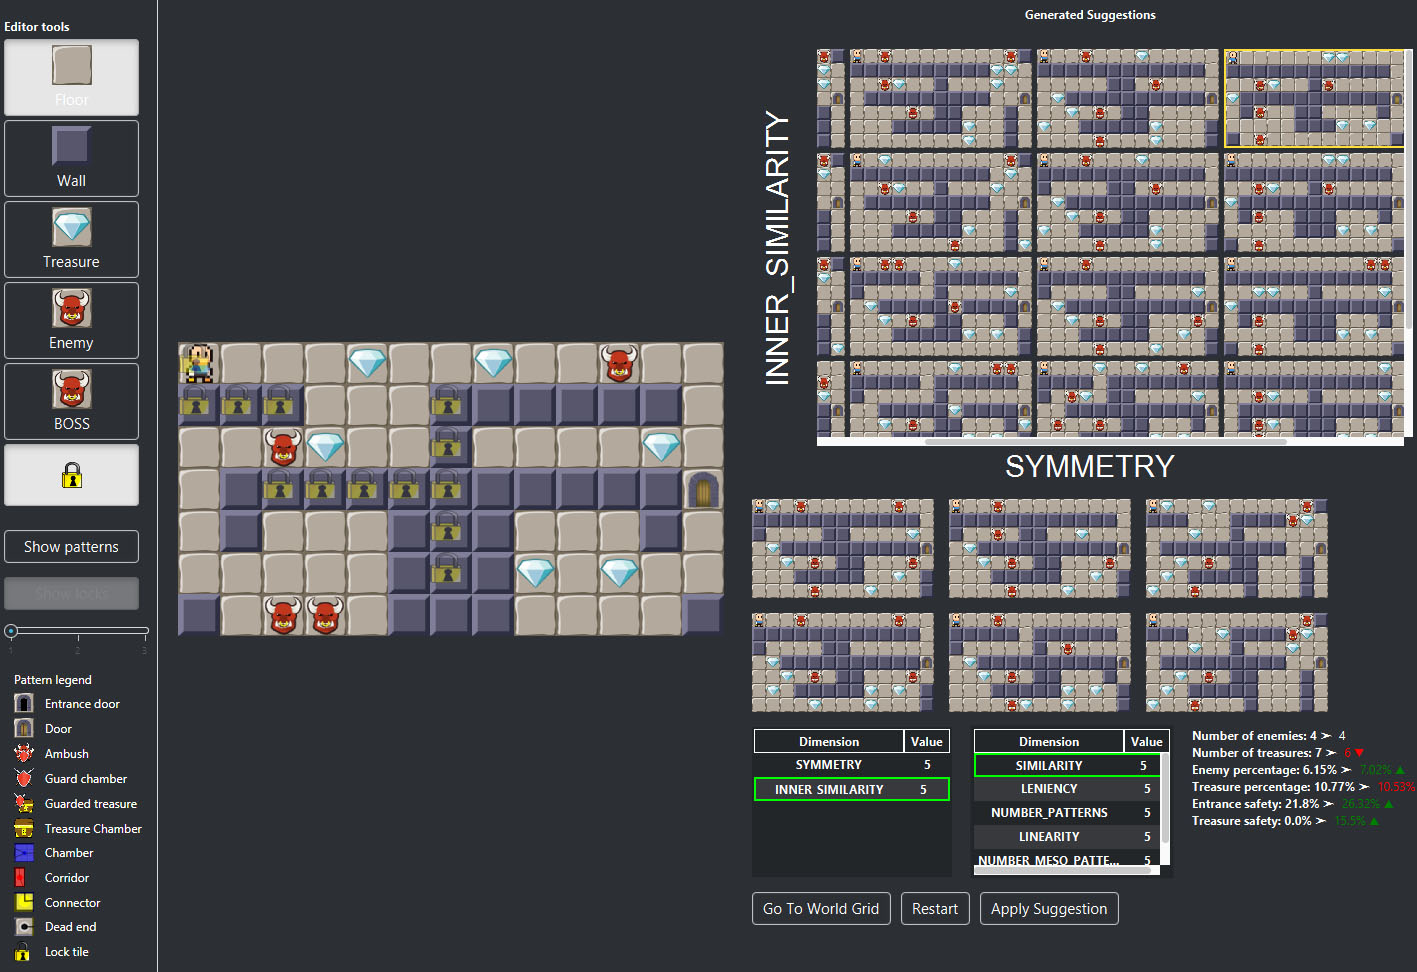
\includegraphics[width=\textwidth]{fig2.jpg}
\caption{The room editor screen in EDD. The top-right pane shows the suggestions provided by the IC MAP-Elites algorithm. Below are the six top-raked suggestions by the Designer Preference Model. The left pane contains the manual edition features.} \label{p5fig2}
\end{figure}

The remaining sections of the paper are structured as follows: Section 3 describes the data-driven Designer Preference Model; Section 4 presents the initial experimental results, and Section 5 discusses the results and future lines of research of this novel approach.

%%Check the section references!